\chapter{An introduction to Zigbee and IEEE 802.15.4}

Zigbee and IEEE 802.15.4 are specifications for the higher and lower network layers of WSNs.\footnote{This chapter is based on \cite{baronti2007wsn} and \cite{farahani2008zwn}}
Zigbee devices are designed for low-range, low-complexity, low-cost and low-consumption applications.
Zigbee includes low duty-cycle capabilities, which mean that the devices can sleep for most of the time.
A zigbee product can potentially run on batteries for years.
In our particular course, we use zigbee combined with Arduino.
As Arduino is not designed for low consumption, it kills the possibility of running our prototypes on batteries for such a long time.

Zigbee defines the network and application layers of the devices and relies on IEEE 802.15.4 for the MAC and PHY layers.
The specification of Zigbee standards is carried out by the Zigbee Alliance, which comprises all kind of companies (semiconductor industry, OEMs, software developers, etc.).
The standardization of IEEE 802.15.4 is done by the IEEE.

\section{IEEE 802.15.4}

\subsection{IEEE 802.15.4 PHY layer}

IEEE 802.15.4 operate in three different bands: 868 MHz (1 channel), 915 MHz (10 channels) and 2.4 GHz (16 channels).
The 2.4 GHz band is a band for industrial, scientific and medical uses (ISM).
This band is shared by many technologies, including the IEEE 802.11 family.
Spread spectrum techniques are used to alleviate the problem of interference.
The modulations that are used are BPSK, ASK and O-QPSK.
Direct sequence spread spectrum (DSSS) or parallel sequence spread spectrum (PSSS) is used.

The functionalities offered by the PHY layer of IEEE 802.15.4 include link quality estimation, energy detection and clear channel assessment.

\subsection{IEEE 802.15.4 MAC layer}

Regarding the MAC layer, the standard differentiates two types of devices: Reduced Function Devices (RFD) and Full Function Devices (FFD).
RFDs are simpler, which means that their power consumption and their price can be lower.
The only role that RFDs can play in a sensor network is that of end devices.
RFDs cannot forward packets of other nodes.

The FFD have extended functionality and can act as end devices and also as network coordinators.
Network coordinators can send beacons for synchronization purposes and provide network join services.
FFDs can also relay packets of other nodes for multi-hop communication.

The standard considers two different alternatives for nodes to communicate: master-slave and peer-to-peer.
In the master-slave situation, the slave communicates only with its master.
There is a WSN coordinator (which has to be a FFD) that decides which of the two alternatives is used.

In the master-slave situation, the master periodically broadcasts a beacon and the slave has to synchronize to the beacon to communicate with the master.
The beacon contains control information about the WSN and also a superframe structure.
The superframe divides the time interval between two beacons in three different parts:
The Contention Access Period (CAP), the Contention Free Period (CFP) and the inactive period.

In the CAP, the sensors contend for channel access using slotted CSMA/CA. 
In the CFP, some of the nodes are assigned Guaranteed Time Slots (GTS) by the coordinator.
This means that those slots are reserved for a particular sensor, and that sensor can transmit without contending for the channel.
Finally, in the inactive period, the all the nodes can sleep to save power.

The slaves only have to wake up to receive the beacons and to transmit or receive data.
The master uses the beacon to indicate which of the slaves have data to be delivered.

\section{Devices}

There are two different types of devices: full-function devices (FFD) and reduced-function devices (RFD).
FFDs are more powerful and can assume any role in the network.
RFDs are simpler, and can assume only the role of ``Device'' in the IEEE 802.15.4 terminology (equivalent to ``ZigBee End Device'' in the ZigBee terminology.

The other two possible roles, that can be assumed only by FFDs are ``Coordinator'' and ``PAN Coordinator'' in the IEEE 802.15.4 terminology.
These are equivalent to ``ZigBee Router'' and  ``ZigBee Coordinator'' in the ZigBee terminology.

A ZigBee End Device can be the source or destination of a packet, but it cannot forward packets for other nodes.
A ZigBee Router can relay packets of other nodes.
And a ZigBee Coordinator is the head of the network.
In every every network, there is one and only one Coordinator.

Regarding the topologies, we can consider three different cases: star, tree and mesh.

\section{Channel Access}

In IEEE 802.15.4 there are two methods for networking: beacon-enabled networking and non-beacon networking.
In beacon-enabled networking the coordinator transmits periodical beacons to synchronize the network.
In these beacons, it is possible to define a super-frame structure.
The super-frame structure spans the channel time between two consecutive beacons, and differentiates three periods: Contention Access Period (CAP), Contention Free Period (CFP, optional) and Inactive Period (IP, optional).
The time is divided in slots, and multiple slots can be assigned to each of the different periods.
In the CAP, the devices use CSMA/CA to contend for channel access.
In the CFP, the channel time is reserved and only the devices that own the reservation can transmit.
In the IP, the devices can go to sleep to save energy.

In non-beacon networking, the devices must always contend for the channel.
The contention uses the CSMA/CA protocol.
Before transmitting, the devices sense the channel for the presence of an ongoing transmission.
If a transmission is detected, the devices backs off and re-attempts after a random period of time.

There are two mechanism to detect an ongoing transmission.
Energy detection in which the device simply measures the amount of energy on the channel,
and carrier detection in which the device looks for the presence of an IEEE 802.15.4 carrier.
Either one or the other, or even a combination of both, can be used.

\section{MAC handshake}

In a beacon-enabled network, a node that wants to transmit data to the coordinator waits for the CFP if it has a reservation.
Otherwise, it waits for the CAP.
Then it transmits the packet (using CSMA/CA if it is in contention mode).
The sender can request acknowledgement and, in this case, the coordinator may acknowledge the reception.

When a coordinator wants to transmit data to a device it indicates in the beacon the destination of the packet.
The device processes the beacon and learns that there is data pending for it.
After that, the device sends a ``data request'' message to the coordinator that the coordinator must acknowledge.
Then the coordinator sends the data packet to the device which may acknowledge the correct reception.

In a non-beacon network, a device can transmit to the coordinator whenever the channel is sensed empty.
If a coordinator has data for a device, it waits until the device sends a ``data request'' which must be acknowledged.
Then the coordinator sends the data to the device, that may acknowledge the correct reception.

\section{MAC problems in multi-hop wireless networks}

There are two well-known problems that recurrently appear in multi-hop wireless networks.
The first one is the ``hidden node problem'' and is represented in Figure \ref{fig:hidden}.
Imagine that nodes $A$ and $C$ cannot carrier sense each other. 
Then it can happen that $C$ starts a transmission while $A$ is transmitting to $B$.
This results in a collision and the receiver may not be able to recover any of the packets.

\begin{figure}[htbp]
  \centering
  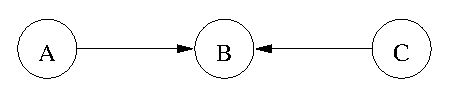
\includegraphics[height=0.1\linewidth]{figures/hidden.eps}
  \caption{Hidden node problem}
  \label{fig:hidden}
\end{figure}

The other problem is the ``exposed node problem'', illustrated in Figure \ref{fig:exposed}.
In the example, $E$ is transmitting to $D$.
Node $F$ wants to transmit to $G$, but it senses the channel busy (as it detects $E$'s transmission).
$F$ does not transmit when, in fact, it could transmit without interfering with the other transmission.
\begin{figure}[htbp]
  \centering
  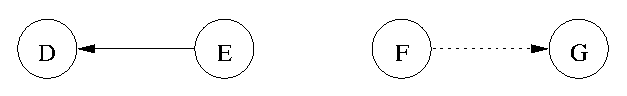
\includegraphics[height=0.1\linewidth]{figures/exposed.eps}
  \caption{Exposed node problem}
  \label{fig:exposed}
\end{figure}

\section{Addresses and Network Layer}

Each device has two addresses: a 16 bit short address and a 64-bit extended address.
